%no borrar PREAMBULO
\documentclass[12pt]{article}

\usepackage[top=3 cm, bottom=2.5  cm, left=2.5 cm, right=2.5 cm]{geometry}
\usepackage{fancyhdr}
\pagestyle{fancy}

\usepackage[hidelinks]{hyperref} %esta opción saca las cajas de colores de los hiperlinks

\fancyfoot[C]{\thepage }  %numera las páginas

\usepackage[utf8]{inputenc}

\usepackage{amsmath,amsfonts,amssymb}
\usepackage{xcolor}
\usepackage{fancyvrb}
\newcommand\verbbf[1]{\textcolor[rgb]{0,0,1}}%comando para colorear el texto en verbatim

%\linespread{1} %por si queremos achicar el espacio entre lineas

\usepackage{tabularx,booktabs}
\usepackage{graphicx}
\usepackage{float} %para que las figuras puedan ponerse en cualquier lado

\usepackage{subcaption}
\usepackage{layout}
\usepackage{multicol}  %para escribir en columnnas 
\usepackage{float}
\usepackage{textcomp}
\usepackage{natbib}
\usepackage{tikz}
\usepackage{multirow} %para cambiar el alto de una fila en una tabla
\tikzset{
  connect/.style = { dashed, gray }
}
\usepackage{pgfplots}
\pgfplotsset{compat=1.8}
\usepackage[english ,spanish]{babel}
\usepackage{latexsym}
\usepackage{verbatim}

%\usepackage{alltt}
\usepackage{indentfirst}

\usepackage{fancybox, calc} 

\usepackage[flushmargin]{footmisc} %para alinear las notas de página

\usepackage{url}
\usepackage{advdate}
\usepackage{wrapfig}
\usepackage{amsthm}
\usepackage[inline]{enumitem} %para hacer listas en una linea, los mismos comandos con *
\newtheorem*{myteo}{Teorema} % la * es para no numerarlos
\newtheorem*{myexample}{Ejemplo}
\newtheorem*{myprop}{Proposición}
\newtheorem*{mylem}{Lema}
\theoremstyle{definition}
\newtheorem*{mydef}{Definición}
\newtheorem{ejer}{Ejercicio}
\newtheorem*{mydefs}{Definiciones}
%\theoremstyle{remark}
\newtheorem*{myobs}{Observación}
\newtheorem*{remark}{Importante}

\renewcommand{\baselinestretch}{1}  %interlineado

\addto\captionsspanish{%
  \renewcommand{\figurename}{Figura}%
}

\newcommand\myText[1]{\text{\scriptsize\tabular[t]{@{}l@{}}#1\endtabular}}
\addto\captionsspanish{%
  \renewcommand{\tablename}{Tabla}%
}

\def \ds {\displaystyle} %define un comando abreviado  
\def\com{“R”}

\usepackage{hyperref}%para referencias de internet con link!
\newcommand*{\fullref}[1]{\hyperref[{#1}]{ \nameref*{#1}}}
%comando \fullref para que ademas del número de capitulo, sección etc. escriba el título del capitulo, sección o lo que sea a lo que estamos haciendo referencia

\newcommand\comentario[1]{\textcolor{red}{#1}}%comentarios en el pdf

\interfootnotelinepenalty=10000 %previene que se pasen a otra página las notas de pie
\raggedbottom 
\addtolength{\topskip}{0pt plus 10pt}
\addtolength{\footnotesep}{0.1mm}

\VerbatimFootnotes%para poder usar Verbatim en las notas de pie

\begin{document}

\fancyhf{}
\pagestyle{fancy}
\lhead{Departamento de Matem\'{a}tica\\Universidad Nacional del Comahue}
\rhead{Matem\'{a}tica 1\\ Licenciatura en Ciencias Biol\'{o}gicas}

%HASTA ACA 

\begin{centering}
\Large{\textbf{Trabajo Práctico N° 5}}\\
\large{\textbf{Límite de sucesiones}}\\
\end{centering}
\vspace{1cm}

%Definicion de sucesión
\fbox{ \parbox{0.98\linewidth}{
\noindent
\begin{mydef}  \textbf{Sucesión.}\\
\noindent
Se define como sucesión de números reales a una función con dominio en el conjunto de los números naturales y codominio en el conjunto de los números reales, es decir:
%\begin{equation*}
\begin{align*}
f:& \mathbb{N} \to \mathbb{R}\\
& n \to f(n)
\end{align*}
%\end{equation*}
\end{mydef}
}}


\begin{enumerate}

\item Calcular los diez primeros términos de las siguientes sucesiones y graficarlas (podés usar Excel, por ejemplo):

\begin{equation*}
a(n) = \frac{(-1)^n}{n} \qquad \qquad
b(n)= 
\begin{cases} 
 1 & \text{si  n es impar} \\
 2n^2 & \text{si  n es par}
\end{cases} \qquad \qquad
c(n) = 2n + 1
\end{equation*}

%2
\item Las siguientes secuencias representan los primeros términos de distintas sucesiones. Hallar una expresión formal para el término general $a(n)$ de cada una de ellas. Bosquejar un gráfico. (También se puede usar Excel, Graph o similar para graficar).
\begin{multicols}{3}
\begin{enumerate}
\setlength\itemsep{0em}
\item $2,4,6,8,10, ...$
\item $2,4,8,16,32, ...$
\item $1,3,5,7,9, ...$
\item $3,9,27,81,...$
\item $3,5,7,9,11, ...$
\item $1,4,9,16,25,36, ...$
\item $ 0,2,4,6,8, ...$
\item $1,8,27,64,125, ...$ 
\item $5, 7, 9, 11,13, ...$
\item $ 10, 15, 20,25, ...$
\item $3, 6, 9, 12,15, ...$
\item $-1, 1, -1, 1, -1, 1, ...$
\item $1, -1, 1, -1, 1, -1, ...$
\item $0, 2, 0, 4, 0, 8, 0, 16, ...$
\end{enumerate}
\end{multicols}

%3
\item Bajo condiciones ideales una célula puede dividirse en dos células hijas en un cierto intervalo de tiempo $t$. Las nuevas células, una vez que transcurre otro intervalo de duración $t$, vuelven a subdividirse en dos células hijas cada una. Supongamos que el tiempo se mide en unidades que coinciden con la duración $t$ del intervalo.
\begin{enumerate}
\setlength\itemsep{0em}
\item Escribir los números de células esperables después de $1, 2, 3, 4...$ unidades de tiempo.
\item Llamando $C(n)$ al número de células en el tiempo $n$ (después de n intervalos de duración $t$), encontrar una expresión general para el número de células en función del tiempo.
\item Graficar esta función. 
\item ¿Es una sucesión? ¿Por qué?
\end{enumerate}
 
%4
\item El isótopo radioactivo del carbono $C^{14}$ tiene una vida media de $5760$ años, lo cual significa que si $N$ es la cantidad de átomos de  $C^{14}$, transcurridos $5760$ años, $N$ se verá reducido a la mitad. Supongamos que consideramos intervalos de tiempo de $5760$ años de duración. Llamando $N_0$ a la cantidad de átomos de carbono cuando $t = 0$, se pide:
\begin{enumerate}
\setlength\itemsep{0em}
\item Escribir los números de átomos esperables después de $1, 2, 3, 4...$ unidades de tiempo.
\item Llamando $N(t)$ al número de  de átomos en el tiempo $t$ (después de $t$ intervalos de $5760$ años de duración), encontrar una expresión general para el número de átomos en función del tiempo.
\item Graficar esta función. 
\item ¿Es una sucesión? ¿Por qué?
\end{enumerate}


%5
\item Para cada una de las siguientes sucesiones, cuyos términos generales se escriben a continuación, se pide:
\begin{enumerate}
\setlength\itemsep{0em}
\item Escribir los diez primeros términos de cada una.
\item Realizar un gráfico de estas sucesiones y comparar sus “comportamientos”. ¿Cómo podría describirse cada uno de ellos?
\item Proponer otros tres ejemplos de sucesiones que tengan comportamientos similares a los dados. 
\noindent
\end{enumerate}
%%
\begin{equation*}
a(n) = 2 + \frac{1}{n} \qquad \qquad
b(n)= 
\begin{cases} 
1 & \text{si  n es impar} \\
n^2 & \text{si  n es par}
\end{cases} \qquad \qquad
c(n) = 2n^2 -4
\end{equation*}

\vspace{1 cm}

\fbox{ \parbox{0.98\linewidth}{
\noindent
Sin pensar en una definición formal, podríamos decir intuitivamente que a las sucesiones que tienen un comportamiento como $c(n)$ del ejercicio anterior, en la que los términos son más y más grandes a medida que se toma $n$ mayor, se las denomina \textit{divergentes}. Si en cambio cuando $n$ crece, los términos de la sucesión se acercan cada vez más a cierto valor $L$, como es el caso de la sucesión $a(n)$, se la llama sucesión \textit{convergente}. El caso de la sucesión $b(n)$ es el de una sucesión que no converge ni diverge, pues no posee un comportamiento similar ni al de $a(n)$ ni al de $c(n)$. (Se las denomina  \textit{oscilantes}, sin que esto signifique que hay una oscilación en el sentido físico del término.)
}}

\vspace{1 cm}
%6
\item Según este criterio, ¿cómo podrían clasificarse las sucesiones del ejercicio 2?

\vspace{1cm}



\vspace{0.5 cm}
%Definicion de sucesión convergente
\fbox{ \parbox{0.98\linewidth}{
\noindent
\begin{mydef}  \textbf{Sucesión convergente.} \\
\noindent
Una sucesión $a(n)$ se dice convergente al número real $L$ si, para cualquier distancia $\epsilon>0$, es posible determinar un número natural $N(\epsilon)$ de modo que si $n$ es tomado mayor que $N(\epsilon)$, entonces la distancia entre $a(n)$ y $L$ será menor que $\epsilon$.  \\
Es decir: \\
\begin{minipage}[b]{1\linewidth}
\begin{center}
$a(n)$ \textbf{converge} a $L$ si parar todo $\epsilon>0$,\\ 
existe $N(\epsilon)$ tal que, si $n > N(\epsilon)$, entonces $|a(n) - L| < \epsilon$ 
\end{center}
\end{minipage}
\vspace{0.5 cm}
\\
Si $a(n)$ converge a $L$ se dice que $a(n)$ \textbf{tiene límite $L$} y se escribe:
\begin{equation*}
\lim_{n \to \infty} a(n) = L
\end{equation*}
\end{mydef}
}}
\vspace{0.5 cm}
%7
\item Explicar en términos de distancia el significado de la desigualdad $|a(n) - L| < \epsilon$.

%8
\item Analizar el siguiente razonamiento y decir si es correcto o no. Fundamentar. \\
“De cierta sucesión $a(n)$ se sabe que si $n$ se toma mayor que $345$, la distancia entre $a(n)$ y $4$ es menor que $0,0001$, si $n$ se toma mayor que $1525$, la distancia entre $a(n)$ y $4$ es menor que $0,00001$, y si $n$ se toma mayor que $9110$, la distancia entre $a(n)$ y $4$ es menor que $0,00000001$. Por lo tanto, la sucesión $a(n)$ converge a $4$."

%9
\item  ¿Por qué en la definición de sucesión convergente es necesario afirmar que \textit{para toda distancia elegida}  $\epsilon>0$, es posible determinar un número naturall $N(\epsilon)$ que cumple con la condición establecida? ¿No sería suficiente con probar que “funciona” para algunos valores de  $\epsilon$? 

%10
\item Para la siguiente sucesión, establecer qué valor o valores de $N(\epsilon)$ "sirven" de acuerdo a la definición de convergencia para el $\epsilon$ marcado:
\begin{figure}[H]
\centering
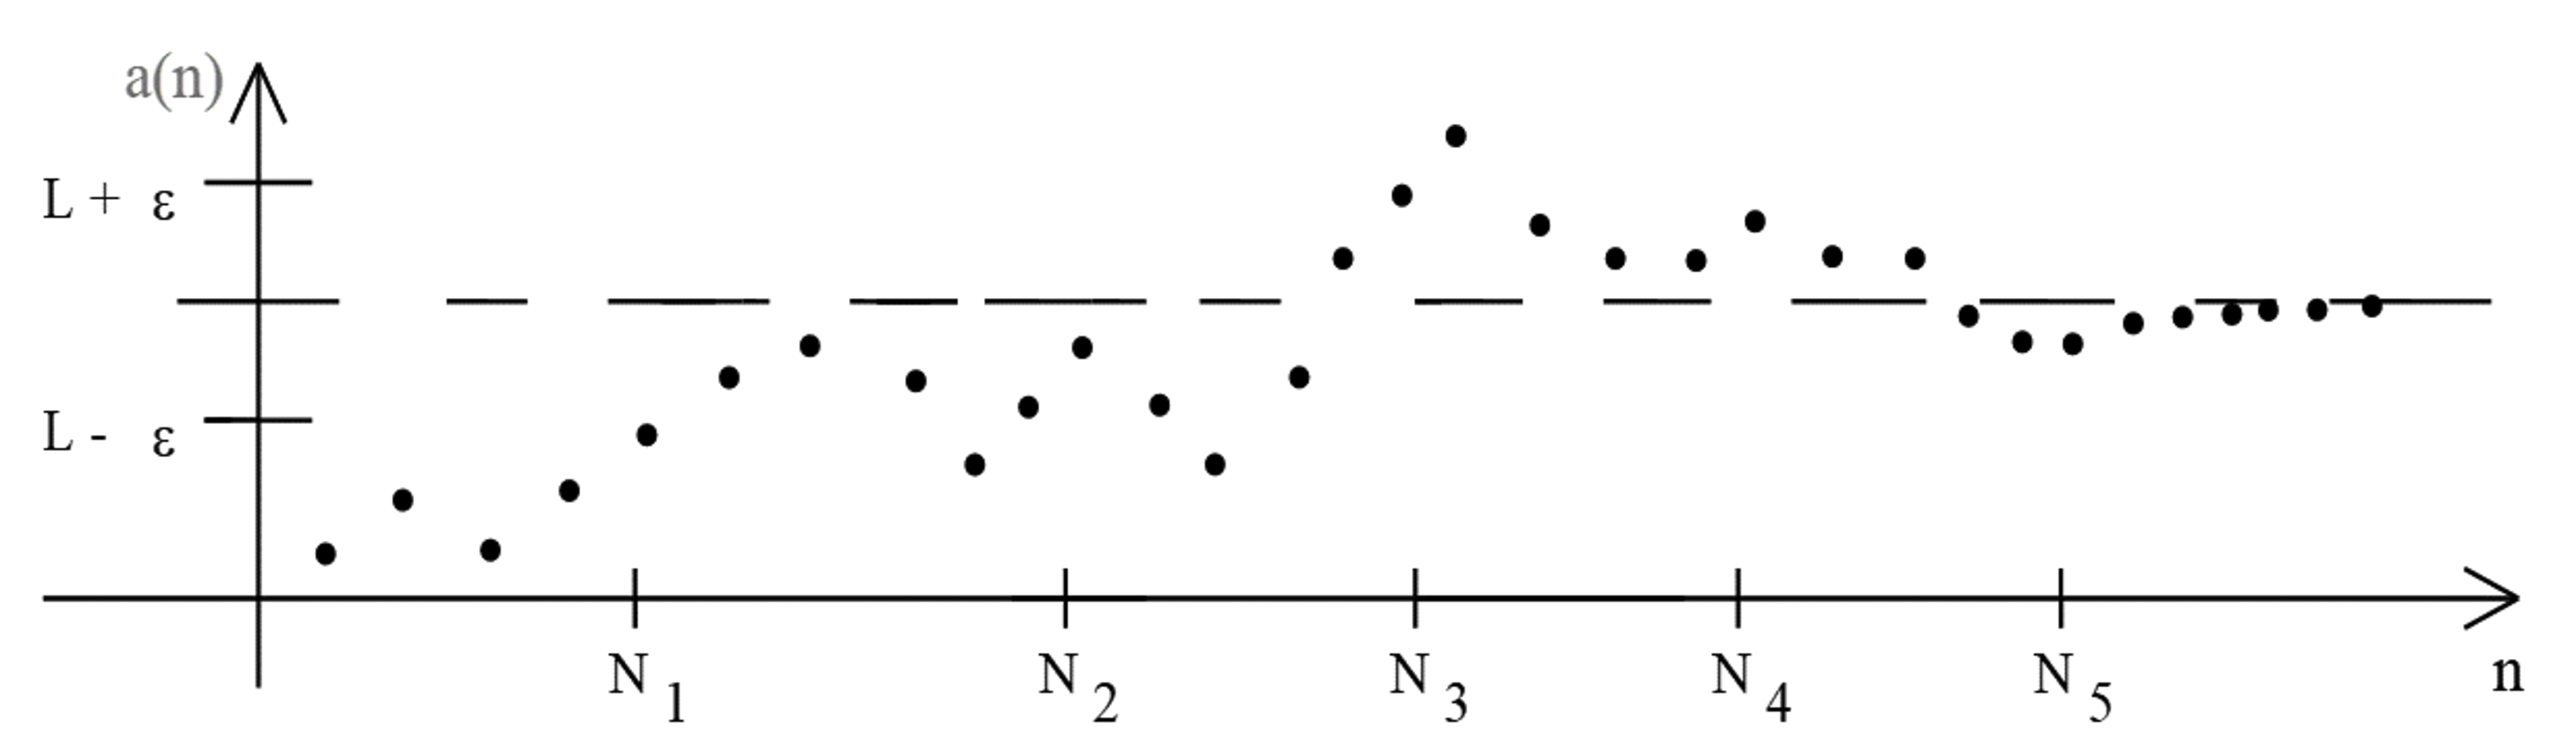
\includegraphics[width=0.9\textwidth]{TP3Fig1}
\end{figure}

%11
\item Para la siguiente sucesión, establecer qué valor o valores de $\epsilon$ pueden corresponder de acuerdo a la definición de convergencia para el  $N(\epsilon)$ elegido:
\begin{figure}[H]
\centering
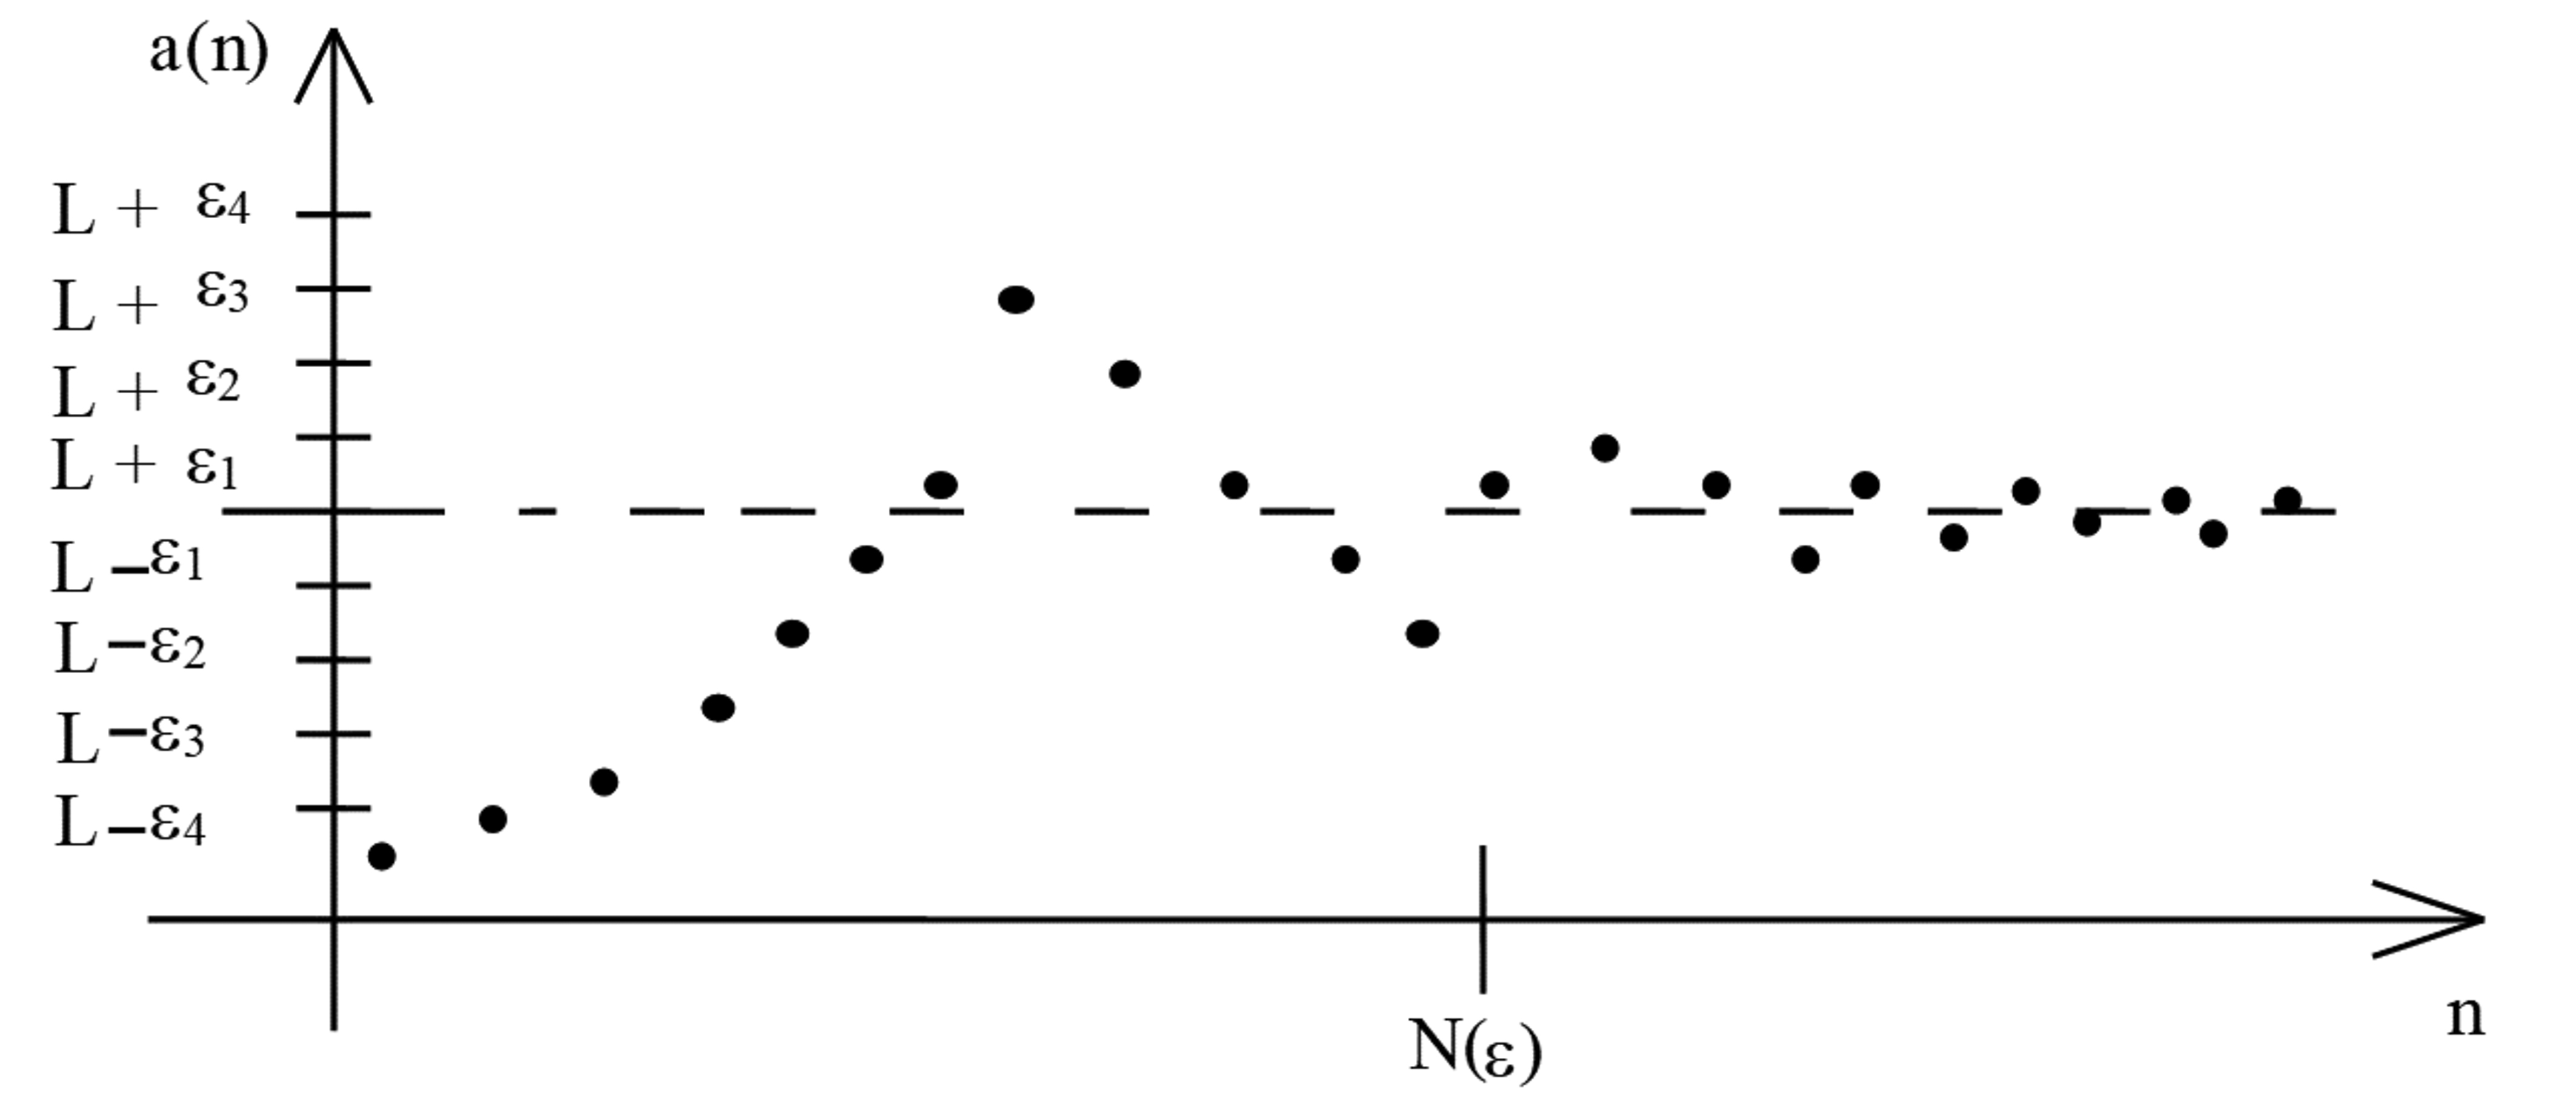
\includegraphics[width=0.9\textwidth]{TP3Fig2}
\end{figure}

%Definicion de sucesión divergente
\fbox{ \parbox{0.98\linewidth}{
\noindent
\begin{mydef}  \textbf{Sucesión divergente.} \\
\noindent
Una sucesión $a(n)$ se dice divergente si para cualquier distancia $K>0$, es posible determinar un número natural $N(K)$ de modo que si $n$ es tomado mayor que $N(K)$, entonces el valor absoluto de $a(n)$ será mayor que $K$.  \\
Es decir: \\
\begin{minipage}[b]{1\linewidth}
\begin{center}
$a(n)$ \textbf{diverge} si para todo $K>0$,\\ 
existe $N(K)$ tal que, si $n > N(K)$, entonces $|a(n)| > K$ 
\end{center}
\end{minipage}
\vspace{0.5 cm}
\\
Si $a(n)$ diverge, se dice que \textbf{tiene límite infinito} y se escribe:
\begin{equation*}
\lim_{n \to \infty} a(n) =  \infty
\end{equation*}
\end{mydef}
}}
\vspace{0.5 cm}

%12
\item Explicar en términos de distancia el significado de la desigualdad $|a(n)| > K$ .

%13
\item Analizar el siguiente razonamiento y decir si es correcto o no. Fundamentar.\\
“De cierta sucesión $a(n)$ se sabe que si $n$ se toma mayor que $1230$, $a(n) > 10000$, si $n$ se toma mayor que $4125$, $a(n) > 100000$, si $n$ se toma mayor que $9372$, $a(n) > 10000000$. Por lo tanto, la sucesión es divergente”.

%14
\item Para la siguiente sucesión, establecer qué valor o valores de $N(K)$ "sirven" de acuerdo a la definición de divergencia para el $K$ marcado:

\begin{figure}[H]
\centering
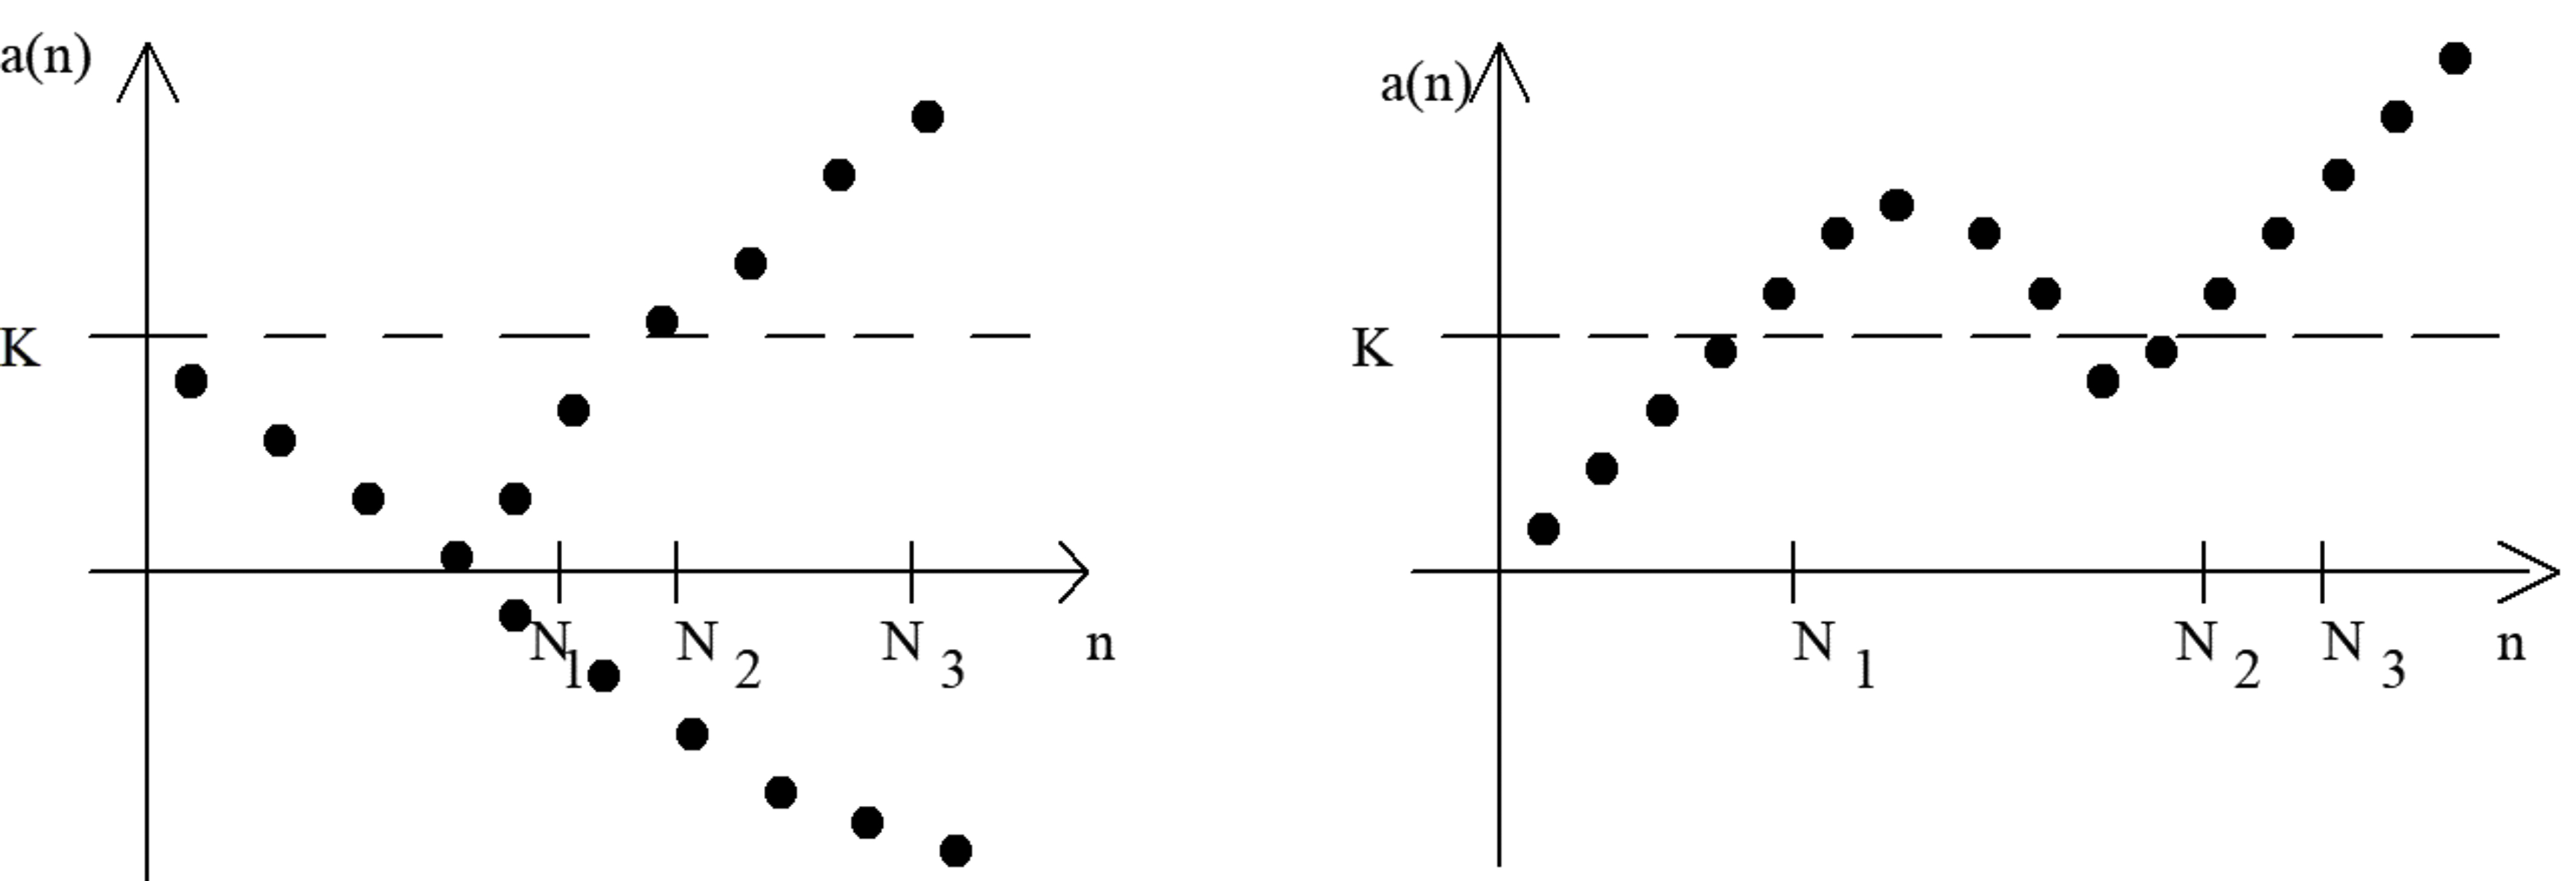
\includegraphics[width=0.9\textwidth]{TP3Fig3}
\end{figure}

%15
\item Para la siguiente sucesión, establecer qué valor o valores de $K$ pueden corresponder de acuerdo a la definición de divergencia para el $N(K)$ marcado:
\begin{figure}[H]
\centering
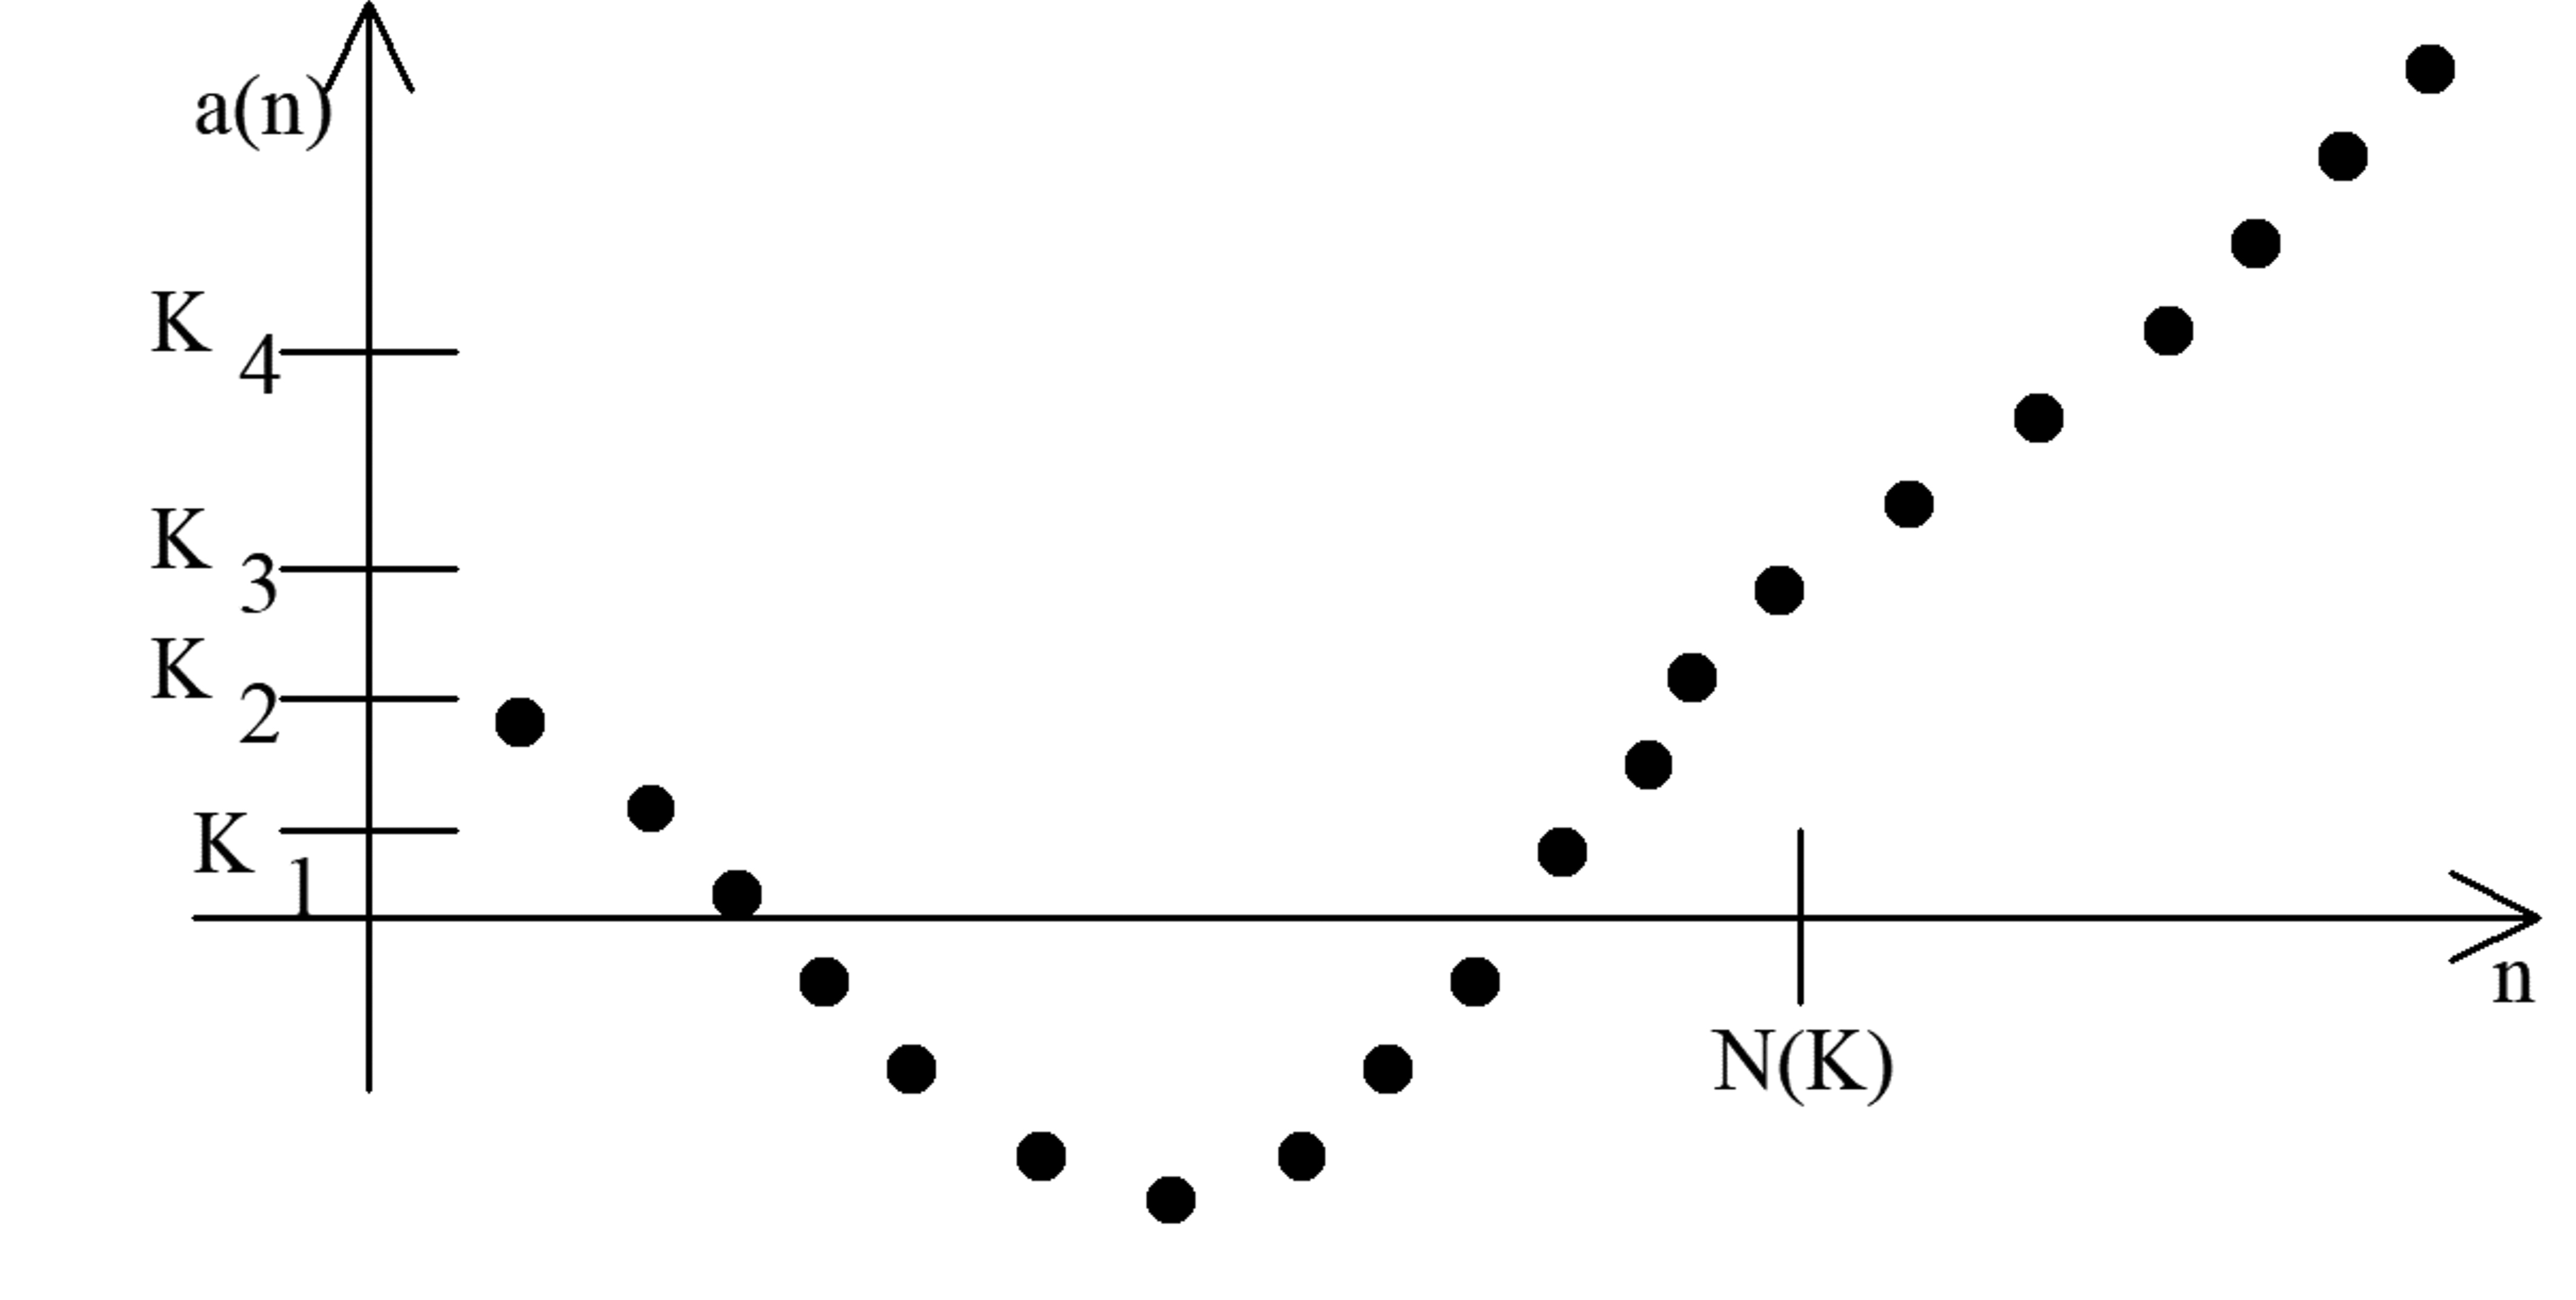
\includegraphics[width=0.9\textwidth]{TP3Fig4}
\end{figure}

%Definicion de sucesión oscilante
\fbox{ \parbox{0.98\linewidth}{
\noindent
\begin{mydef}  \textbf{Sucesión oscilante.} \\
\noindent
Llamaremos oscilantes, a todas aquellas sucesiones que no convergen ni divergen.
Una sucesión se dice oscilante si existen al menos dos subsucesiones con distinto límite (uno finito y el otro infinito o ambos finitos y distintos).\\
Una sucesión oscilante se dice que no tiene límite (ni finito ni infinito).
\end{mydef}
}}
\vspace{0.5 cm}

%Definicion de sucesiones acotadas
\fbox{ \parbox{0.98\linewidth}{
\noindent
\begin{mydef}  \textbf{Sucesión acotada.} \\
\noindent
Una sucesión $a(n)$ se dice  \textbf{acotada superiormente}, si existe un valor $C \in \mathbb{R}$ tal que para todo valor de $n$, las imágenes de la sucesión son menores o iguales que $C$. En símbolos:\\
\begin{minipage}[c][1 cm]{1\linewidth}
\begin{center}
$a(n)$ es \textbf{acotada superiormente} si existe $C \in \mathbb{R}$, tal que para todo $n$, $a(n) \leq C$ 
\end{center}
\end{minipage}
\noindent
Una sucesión $a(n)$ se dice  \textbf{acotada inferiormente}, si existe un valor $c \in \mathbb{R}$ tal que para todo valor de $n$, las imágenes de la sucesión son mayores o iguales que $c$. En símbolos:\\
\begin{minipage}[c][1 cm]{1\linewidth}
\begin{center}
$a(n)$ es \textbf{acotada inferiormente} si existe $c \in \mathbb{R}$, tal que para todo $n$, $a(n) \geq  c$ 
\end{center}
\end{minipage}

\noindent
Una sucesión que es a la vez acotada superior e inferiormente, se dice \textbf{acotada}.
\end{mydef}
}}
\vspace{0.5 cm}

%16
\item Proponer ejemplos gráficos de sucesiones acotadas superior pero no inferiormente, acotadas inferior pero no superiormente, y sucesiones acotadas (tanto superior como inferiormente).

%17
\item Para cada una de las siguientes sucesiones realizar un bosquejo (aproximado) de las mismas (podés usar cualquier graficador). A continuación:
\begin{enumerate}
\setlength\itemsep{0em}
\item Decidir si es o no acotada (superior y/o inferiormente).
\item Establecer la mínima cota superior y/o máxima cota inferior, si existen. 
\item Pensar si existen otras cotas. Ejemplificar.
\item ¿Es alguna de las sucesiones convergente o divergente?
\item ¿Es posible establecer alguna relación entre convergencia y divergencia de una sucesión y el hecho de que sea o no acotada? Si es posible, establecer una regla general.
\end{enumerate}
\begin{equation*}
a(n) = \frac{n-3}{n^2+1} \qquad\qquad
b(n)= log(n+3)\qquad\qquad
c(n) = \frac{2n+3}{n+1}
\end{equation*}

\vspace{0.3 cm}

\fbox{ \parbox{0.98\linewidth}{
\noindent
\begin{myteo}
Toda sucesión convergente es acotada.
\end{myteo}
}}

\vspace{0.5 cm}

%18
\item  Enunciar la afirmación recíproca del teorema anterior ($q\Rightarrow p$). ¿Es verdadera o falsa? Proponer ejemplos de sucesiones que lo muestren.	

\fbox{ \parbox{0.98\linewidth}{
\noindent
\begin{myteo}
Toda sucesión divergente es no acotada.
\end{myteo}
}}
\vspace{0.5 cm}

%19
\item ¿Cuáles pueden ser, en este teorema, las posibilidades para “no acotada”?


%20
\item Enunciar la afirmación recíproca del teorema anterior  ($q\Rightarrow p$). ¿Es verdadera o falsa? Proponer ejemplos de sucesiones que lo muestren.


%21
\item Proponer ejemplos gráficos de sucesiones covergentes tales que:
\begin{enumerate}
\setlength\itemsep{0em}
\item el límite coincida con alguna cota superior.
\item el límite coincida con alguna cota inferior.
\item el límite no coincida con ninguna cota.
\end{enumerate}
	
\fbox{ \parbox{0.98\linewidth}{
\noindent
\begin{myteo}[Teorema del \textit{sandwich}.] 
Sean dos sucesiones $a(n)$ y $b(n)$, convergentes al mismo valor $L$, es decir, 
\begin{equation*}
\lim_{n \to \infty} a(n) =  \lim_{n \to \infty} b(n) = L
\end{equation*}
y una tercera sucesión $c(n)$, para las que a partir de determinado valor de $n$, llamémoslo $N$, se cumple que $a(n) \leq c(n) \leq b(n)$. Entonces:
\begin{equation*}
\lim_{n \to \infty}c(n) =  L
\end{equation*}
\end{myteo}
}}
\vspace{0.5 cm}

%22
\item Interpretar gráficamente el teorema anterior y explicar.

%23
\item Hacer un gráfico de las siguientes sucesiones (por separado) que muestre aproximadamente su comportamiento. ¿Qué puede decirse acerca de la convergencia o divergencia de las mismas?
\setlength\itemsep{0em}

\begin{equation*} 
a(n)= 
\begin{cases} 
 \frac{1}{n} & \text{si }  n \leq 10^3 \\
n & \text{si }  n >10^3
\end{cases} \qquad
\begin{cases} 
 \frac{1}{n}  & \text{si  n es impar} \\
 \frac{1}{2n}  & \text{si  n es par}
\end{cases} \qquad
\begin{cases} 
 \frac{1}{3n-2} & \text{si }  n \leq 50 \\
 n.[(-1)^n +1] & \text{si } n > 50
\end{cases}
\end{equation*}
	
\fbox{ \parbox{0.98\linewidth}{

\begin{myteo}
Para las sucesiones convergentes se tiene que:\\
\begin{enumerate}
\setlength\itemsep{0em}
\item La suma de dos sucesiones convergentes es otra sucesión convergente, y el límite de la suma es la suma de los límites de ambas sucesiones.
\item El producto de una sucesión convergente por una constante $k \in \mathbb{R}$ es también convergente, y el límite es igual a k por el límite de la sucesión.
\item El producto de dos sucesiones convergentes es otra sucesión convergente y el límite del producto es el producto de los límites de ambas sucesiones.
\item El cociente de dos sucesiones convergentes es otra sucesión convergente, y el límite del cociente es el cociente de los límites de ambas sucesiones, siempre que la sucesión del denominador no converja a $0$.
\end{enumerate}

En símbolos, sea $k$ un número real y sean dos sucesiones $a(n)$ y $b(n)$, convergentes a $L$ y $M$ respectivamente. Es decir:
\begin{equation*}
\lim_{n \to \infty} a(n) = L  \qquad \text{y} \qquad \lim_{n \to \infty} b(n) = M
\end{equation*}

Entonces: 

\begin{enumerate}
\setlength\itemsep{0em}
\item 
$\lim\limits_{n \to \infty} \left[a(n) + b(n)\right] =  \lim\limits_{n \to \infty} a(n) +  \lim\limits_{n \to \infty} b(n) = L + M$
\item 
$\lim\limits_{n \to \infty} k.a(n) = k.  \lim\limits_{n \to \infty} a(n) = k. L$
\item 
$\lim\limits_{n \to \infty} a(n). b(n)=  \lim\limits_{n \to \infty} a(n). \lim\limits_{n \to \infty} b(n) = L.M$
\item 
$\lim\limits_{n \to \infty} \frac{a(n)}{b(n)}=  \frac{\lim\limits_{n \to \infty} a(n)}{ \lim\limits_{n \to \infty} b(n)} = \frac{L}{M} , \; \text{siempre que } M \neq 0.$
\end{enumerate}

\end{myteo}
}}

%%%

\vspace{0.5 cm}

\fbox{ \parbox{0.98\linewidth}{

\begin{myteo} Si la sucesión $a(n)$ converge a $0$, la sucesión $b(n) =  \frac{1}{a(n)}$  diverge, es decir: 
\begin{equation*}
 \text{Si }\lim_{n \to \infty} a(n) = 0 \text{, entonces }   \lim_{n \to \infty} \frac{1}{a(n)} =  \infty
\end{equation*}
\end{myteo}
}}


%24
\item Mostrar un ejemplo de una sucesión que converja a $0$ y verificar que su recíproca diverge.

\vspace{0.5 cm}

\fbox{ \parbox{0.98\linewidth}{

\begin{myteo} Si la sucesión $a(n)$ diverge, la sucesión $b(n) =  \frac{1}{a(n)}$  converge a $0$, es decir: 
\begin{equation*}
 \text{Si }\lim_{n \to \infty} a(n) =  \infty \text{, entonces }   \lim_{n \to \infty} \frac{1}{a(n)} = 0
\end{equation*}
\end{myteo}
}}

\vspace{0.3 cm}
%25
\item Mostrar un ejemplo de una sucesión que diverja y verificar que su recíproca converge a $0$.
\vspace{0.5 cm}

\fbox{ \parbox{0.98\linewidth}{
\begin{myteo} Si la sucesión $a(n)$ converge a $L \neq 0$ y  $b(n)$ diverge, entonces su producto diverge. Es decir:
\begin{equation*}
 \text{Si } \lim_{n \to \infty} a(n) = L\neq 0 \; \text{ y } \;  \lim_{n \to \infty} b(n) =  \infty  \text{, entonces }  \lim_{n \to \infty} a(n). b(n)=   \infty 
\end{equation*}
\end{myteo}
}}

\vspace{0.3 cm}
%26
\item Mostrar un ejemplo de una sucesión que converja a $L\neq 0$ y una que diverja y verificar que su producto diverge.
\vspace{0.3 cm}

%Definicion de sucesión
\fbox{ \parbox{0.98\linewidth}{
\noindent
\begin{mydef}  \textbf{Formas indeterminadas.}\\
\noindent
Se denomina \textit{forma indeterminada} o \textit{límite indeterminado}, a un límite del cual es imposible determinar en forma inmediata si es finito, infinito o no existe.\\
Algunas formas indeterminadas son:
\begin{center}
 $\frac{0}{0}$, $\frac{\infty}{\infty}$, $0.\infty$, $0^0$, $1^\infty$, $ \infty^0$, $\infty-\infty$
\end{center}
\noindent
entendiéndose que se trata de una expresión donde participan dos sucesiones que tienden a $0$, $1$ o $\infty$, según corresponda, y no propiamente una operación entre éstos.\\
\textit{Resolver una indeterminación} (o un límite indeterminado), significa llegar a una decisión acerca del límite indeterminado, es decir, poder afirmar si es finito (cuánto vale), es infinito o no existe.
\end{mydef}
}}
\vspace{0.3 cm}


%27
\item Dar ejemplos de sucesiones $a(n)$ y $b(n)$ tales que:\\
\begin{enumerate}
\setlength\itemsep{0em}
\item 
$\lim\limits_{n \to \infty} a(n) =  \lim\limits_{n \to \infty} b(n) = \infty \;\;$ y $\;\; \lim\limits_{n \to \infty} \frac{a(n)}{b(n)} = 3$
\item 
$\lim\limits_{n \to \infty} a(n) =  \lim\limits_{n \to \infty} b(n) = 0 \;\;$ y $\;\; \lim\limits_{n \to \infty} \frac{a(n)}{b(n)} = \infty$
\item 
$\lim\limits_{n \to \infty} a(n)= 0 \;\;$ , $\;\; \lim\limits_{n \to \infty} b(n) = \infty \;\;$ y $\;\; \lim\limits_{n \to \infty} a(n).b(n) \;\;$ no exista.
\item 
$\lim\limits_{n \to \infty} a(n) =  \lim\limits_{n \to \infty} b(n) = +\infty \;\;$ y $\;\; \lim\limits_{n \to \infty} a(n) - b(n) = 2$
\end{enumerate}
\vspace{0.3 cm}

%28
\item Si $a(n)$ y $b(n)$ son dos sucesiones divergentes, ¿se puede afirmar que $a(n) + b(n)$ también es divergente? Ejemplificar. ¿Y si ambas son convergentes?
\vspace{0.5 cm}
%29
\item Decidir el comportamiento de las siguientes sucesiones (es decir, decidir si el límie es finito (y cuánto vale), infinito, o no existe):\\
\begin{multicols}{4}
$a(n) = (2^n)^2$\\\vspace{0.5 cm}
$b(n) = \frac{n-1}{n}$\\\vspace{0.3 cm}
$c(n) = \frac{n+1}{n^2}$\\ \vspace{0.3 cm}
$d(n) = \frac {2^n}{4^n+1}$\\ \vspace{0.3 cm}
$e(n) = \frac{1}{n} - \frac{1}{n+1}$ \\ \vspace{0.3 cm}
$f(n) = (\frac{-1}{2})^n$\\ \vspace{0.3 cm}
$g(n) = \frac{n+(-1)^n}{n}$\\ \vspace{0.3 cm}
$h(n) = 1 + (-1)^n$\\
\end{multicols}

%30
\item
\noindent
Encontrar los valores de $\alpha$ para que la siguiente sucesión resulte a) convergente, b) divergente ó c) oscilante. Justificar
\begin{equation*}
\begin{cases} 
 \frac{1}{n}  & \text{si  n es impar} \\
 e^{2-\alpha^2 n} & \text{si  n es par}
\end{cases}
\end{equation*}


%31
\item En caso de ser posible, complete la siguiente sucesión de modo que (i) converja, (ii) diverja, (iii) oscile. 

\begin{equation*}
\begin{cases} 
 \frac{2n^2+3n-6}{4n^2-2n+2}  & \text{si  n es impar} \\
..............& \text{si  n es par}
\end{cases}
\end{equation*}



%32
\item Considerar la sucesión siguiente y completar de modo que la misma (i) converja, (ii) diverja ó (iii) ninguna de las anteriores. Explicar.

\begin{equation*}
\begin{cases} 
 2n^2-3n+2  & \text{si  ............} \\
2-\frac{1}{n} & \text{si  ............} 
\end{cases}
\end{equation*}



%33
\item En caso de ser posible, complete la siguiente sucesión de modo que (i) converja, (ii) diverja, (iii) oscile. Explicar.

\begin{equation*}
\begin{cases} 
 \frac{2n^3+3n-6}{4n^2-2n+2}  & \text{si  n es impar} \\
..............& \text{si  n es par}
\end{cases}
\end{equation*}

\end{enumerate}

\end{document}
